\subsection{Aufgabe 1}
\begin{figure}[H]
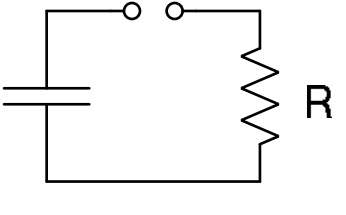
\includegraphics[scale=0.5]{sb1}
\caption{Abbildung 1: Schaltplan Aufgabe 1}
\end{figure}

Für diese Aufgabe wird ein Kondensator mit einem Widerstand in Reihe geschalten (siehe Abbildung 1.1). Mit einem Frequenzgenerator legt man eine Spannung an und mit Hilfe eines Oszilloskops verändert man die Frequenz, bis beide Sinuskurven die gleiche Spannung hatten. Mit einem Spannungsmessgerät (Fluke 175) haben wir die Spannung zwischen dem Widerstand und dem Kondensator gemessen. Dabei betrug der Spannungsunterschied:
\begin{equation}
\notag
\Delta U=0,023 V
\end{equation}

Die Frequenz betrug dabei konstant:

\begin{equation}\notag
f_{char} = (160,45\pm 0,1) Hz
\end{equation}

Die verwendeten Bauteile des R-C-Kreises wurden separat noch einmal nachgemessen, dabei ergab sich für den Widerstand einen Wert von:
\begin{equation}\notag
R = (0.990 \pm 0.012)k\Omega
\end{equation}

und die Kapazität des Kondensators:
\begin{equation}\notag
C = (1.001 \pm 0.013)\mu F
\end{equation}

Die Fehler errechnen sich aus $\pm (1.0\% +3dgt)$.

Nun kann man über folgende Formel den theoretischen Wert der Frequenz f berechnen:
\begin{equation}\notag
f_{theo}=\frac{1}{2\pi RC}= (160.6 \pm 2.0)Hz
\end{equation}

Den Fehler bestimmt man über die Gauß'sche Fehlerfortpflanzung:
\begin{equation}\notag
\Delta f_{theo}=\sqrt{\left(\frac{\partial f_{theo}}{\partial R}\cdot \Delta R\right)^2+\left(\frac{\partial f_{theo}}{\partial C}\cdot \Delta C\right)^2}
\end{equation}

Um nun noch die Phasenverschiebung auszurechnen, benutzt man Gl.\(\eqref{ph}\) und stellen diese nach \(\varphi\) um mit \(\omega=2\pi f_{theo}\)
\begin{equation}\notag
\phi_{theo}=arctan\left(-\frac{1}{\omega RC}\right)=\left(-0,7854 \pm 0.0065\right)^\circ
\end{equation}

Den Fehler bekommt man aus:
\begin{equation}\notag
\Delta \phi_{theo}=\sqrt{\left(\frac{\partial \phi_{theo}}{\partial f_{theo}}\cdot \Delta f_{theo}\right)^2+\left(\frac{\partial \phi_{theo}}{\partial C}\cdot \Delta C\right)^2+\left(\frac{\partial \phi_{theo}}{\partial R}\cdot \Delta R\right)^2}
\end{equation}

\subsection*{Fazit}
Den Wert für die charakteristische Frequenz konnten wir relativ schnell finden, nachdem wir festgestellt hatten, dass ein Messgerät einen Wackelkontakt hatte und bis dahin nur seltsame Werte geliefert wurden.\\
Der theoretische und der gemessene Wert der charakteristische Frequenz sind gleich, nur dass der Fehler des theoretischen Werts aufgrund der Bauteile doch relativ groß ist. Die Phasenverschiebung ist auch ziemlich klein.